\documentclass[a4paper]{article}

\usepackage[utf8]{inputenc}

\usepackage{url}
\usepackage[]{hyperref} %hidelinks

\usepackage{caption}

\usepackage{listings}

\usepackage{color}

% *** GRAPHICS RELATED PACKAGES ***
%\usepackage[pdftex]{graphicx}
\usepackage{graphicx}
%\usepackage[dvips]{graphicx}
% to place figures on a fixed position
\usepackage{float}

\usepackage[margin=1in]{geometry}

\usepackage{enumitem}

\newlist{TASK}{enumerate}{1}
\setlist[TASK]{label=Task-\arabic*:}

\title{OpenFlow \& Mininet – template}
\author{}
\date{}


\begin{document}

\maketitle

\tableofcontents

\section{Introduction}
As computers have become more popular, they have required to be interconnected in order to communicate with each other.
The Internet is a network of autonomous systems (AS) and each AS is a collection of IP networks. Therefore, the
Internet is often called 'the network of networks'. Between autonomous systems, inter-domain routing is used (BGP in
this lab, which is standard for Internet routing), whereas in the AS, intra-domain routing is applied (the widely used
OSPF in this lab). Soon, we will see the interaction of these protocols. The goal of this lab is to show the complexity
of Internet and to present its routing solutions using a simplified model. Please note that the Internet topology and
the number of connections are unknown. There are only approximate data about how billions of hosts are connected to the
global network.

\section{Internet routing}

\subsection{Routing protocol operations; routing table, forwarding table}

In order to have a functional IP routing, each node must have a forwarding table which contains IP prefixes and the
associated next hop addresses. Forwarding table is sometimes called routing table but it can be misleading and it is
important to distinguish these terms. When we send a packet to a destination address, the network layer needs to make a
lookup in the forwarding table. Then the packet is sent to the corresponding IP address. The forwarding table can be
created either manually or by using dynamic routing protocols. A single device may run multiple routing protocols.
These protocols propose changes to the forwarding table but the final decision is made by the network layer of the
device (for instance, the operating system). Each routing process has a separate table which is used to make a
suggestion, also known as the routing table. Although routing processes run on the same device, they don't communicate
with each other by default. As a result, one process doesn't know about routes that other processes have found.
However, we can tell them to exchange routing information and to propagate routes (redistribution). Thus, route
redistribution allows routes from one routing protocol to be advertised into another routing protocol (but it doesn't
mean that each protocol makes the same suggestion to modify the forwarding table). In some cases, redistribution is not
recommended. For example, if a protocol that uses a huge global database injected a large number of routes into a less
scalable interior gateway protocol (IGP), the IGP would be overwhelmed and the routing process would fail.

\subsection{BGP}

Nowadays the Border Gateway Protocol is used on the Internet. BGP is a path-vector routing protocol. It differs from
the distance vector (RIP, EIGRP) and link-state (OSPF) protocols. A BGP routing table entry includes the destination
network (prefix), next-hop address and the path to reach the destination host. When an AS boundary router (ASBR) that
uses BGP receives a path-vector message from an other ASBR, it needs to check the advertised route against its policy.
If the local policy allows the route, the router sends a modified path-vector message to its neighbour: it adds its own
AS number and path information to the message.
BGP was designed to replace Exterior Gateway Protocol (EGP). Due to its hierarchical architecture, EGP can't handle the
routing in modern networks. However, BGP provides distributed operation. It have had many versions since 1994, but the
major enhancement was the support for Classless Inter-Domain Routing (CIDR) and use of route aggregation to decrease
the size of routing tables. Introducing CIDR was inevitable to help slow the rapid exhaustion of IPv4 addresses. Using
CIDR, the division point between the subnet/network ID and the host ID can be on any address bit boundary, instead of
on 8-bit segments. Route aggregation reduces the number of entries in the routing table. Aggregation makes it possible
to advertise many subnets as a single, larger network (super-net). For example, the summary address of 37.0.1.0/24,
37.0.2.0/24...37.0.255.0/24 networks is 37.0.0.0/16. BGP is required of most Internet service providers (ISPs) to
establish routing between one another.

\subsection{BGP operation}

BGP neighbours are established by manual configuration between routers to create a TCP session on port 179. A BGP
speaker sends 19-byte keep-alive messages every 60 seconds to maintain the connection. Among routing protocols, BGP is
unique in using TCP as its transport protocol and also in manual neighbour configuration. In case of interior gateway
protocols, routers become neighbours automatically if possible, whereas BGP requires to configure the neighbour using its
IP address. BGP can be used between different autonomous systems and also between two routers in the same AS. When BGP
runs between two peers in the same AS, it is referred to as Internal BGP (iBGP or Interior Border Gateway Protocol).
When it runs between different autonomous systems, it is called External BGP (eBGP or Exterior Border Gateway
Protocol). Routers on the boundary of one AS exchanging information with another AS are called border or edge routers
or eBGP peers. Please note that IGP and eBGP routes take precedence over iBGP. BGP has optional capabilities including
multi-protocol extensions and various recovery modes. These capabilities can be negotiated during the peering
handshake, when OPEN messages are exchanged. In order to make decisions in its operations with peers, a BGP peer uses a
finite state machine (FSM) that consists of six states. The FSM is shown on Figure~\ref{fig:BGP-FSM}.

\begin{figure}[H]
    \centering
    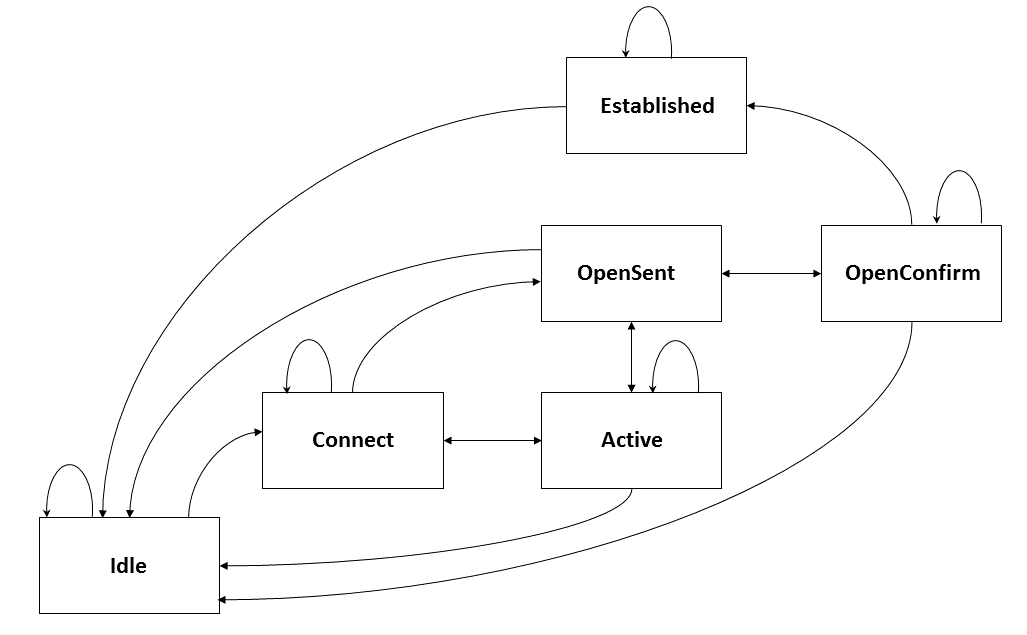
\includegraphics[width=0.9\textwidth]{figures/bgp-fsm.png}
    \caption{BGP neighbouring session establishment state transition diagram}
    \label{fig:BGP-FSM}
\end{figure}

The first state is the "Idle" state. In the "Idle" state, BGP waits for connection attempts from neighbours, initializes
all resources and initiates a TCP connection to the peer. The second state is "Connect". In the "Connect" state, the
router waits for the TCP connection to complete and transitions to the "OpenSent" state if successful. Normally, BGP
does not spend much time in this state. If unsuccessful, it starts a timer and transitions to the "Active" state upon
expiration. In the "Active" state, the router resets the timer to zero and returns to the "Connect" state. If
connection attempts fail many times, it transitions back to "Idle" state. In the "OpenSent" state, the router sends an
Open message and waits for one in return. Once the message has been received, the router checks the validity of the
Open message. If there is no error, a Keep-alive message is sent, various timers are set and the state is changed to
OpenConfirm. If there is an error, the router sends a Notification message to the peer indicating why the error
occurred. In the "OpenConfirm" state, the peer is listening for a Keep-alive message from its peer. If a Keep-alive
message is received and no timer has expired before reception of the Keep-alive, BGP transitions to the "Established"
state. If a timer expires before a Keep-alive message is received, or if an error condition occurs, the router
transitions back to the Idle state. In the "Established" state, the router can send/receive Keep-alive, Update and
Notification messages to/from its peer. If there is any error, BGP transitions back to the "Idle" state. The Update
messages contain information about each route being advertised to the BGP peer. According to the BGP terminology, a
basic CIDR route description is called Network Layer Reachability Information (NRLI). NLRI consists of destination
network prefix, subnet mask, AS path and next-hop address.
All routers within a single AS and participating in BGP routing must be configured in a full mesh: each router must be
configured as peer to every other router. This causes scaling problems, since the number of required connections grows
quadratically with the number of routers involved. To reduce the problem, BGP implements additional options in complex
networks.
A given BGP router may accept NLRI Updates from and advertise to multiple neighbours. BGP maintains its own routing
table, called the Local Routing Information Base (Loc-RIB), separate from the main routing table of the router. For
each neighbour, the BGP process maintains an Adjacent Routing Information Base, Incoming (Adj-RIB-In) containing the
NLRI received from the neighbour, and an Adj-RIB-Out (Outgoing) for NLRI to be sent to the neighbour.
The BGP standard specifies a number of decision factors for selecting NLRI to go into the Loc-RIB. This is more than
the ones that are used by any other common routing process. The first decision point for evaluating NLRI is that its
next-hop attribute must be reachable, so there must be an active route already in the main routing table of the router.
Next, for each neighbour, the BGP process applies various criteria to decide which routes should go into the Adj-RIB.
Only one route to each destination will be installed in the Adj-RIB. This process will also delete any routes from the
Adj-RIB that are withdrawn by the neighbour.
Whenever an Adj-RIB changes, the main BGP process decides if any of the neighbour's new routes are preferred to routes
already in the Loc-RIB. If so, it replaces them. If a given route is withdrawn by a neighbour, and there is no other
route to that destination, the route is removed from the Loc-RIB.
In summary: at the beginning, NLRIs are received and added to the Adj-RIB. After evaluating priorities and policies,
NLRIs go into the Loc-RIB. BGP advertises the Loc-RIB to the main routing table manager which creates the router's
forwarding table.

\section{Router implementation}

\subsection{Cisco IOS}

Cisco IOS is a family of software used on most Cisco routers and network switches. IOS is a package of routing,
switching, inter-networking and telecommunications functions integrated into a multitasking operating system. The IOS
command line interface provides a fixed set of multiple-word commands. The set available is determined by the "mode"
and the privilege level of the current user. "Global configuration mode" provides commands to change the system's
configuration, and "interface configuration mode" provides commands to change the configuration of a specific
interface. All commands are assigned a privilege level from 0 to 15, and can only be accessed by users with the
necessary privilege. Through the CLI, the commands available to each privilege level can be defined.
The required commands for this lab can be found in Section~\ref{sec:further-reading} under Cisco guide.

\subsection{Quagga}
In addition to network device manufacturers, there is an open-source software suite for Linux (Quagga) that implements
dynamic routing protocols. A system with Quagga installed acts as a dedicated router. Quagga supports the most common
IPv4 routing protocols (RIP, OSPF, BGP) and IPv6 protocols as well. The CLI commands are similar to the ones in Cisco
IOS. Routing protocol implementations run in separate daemon processes:
\begin{itemize}
    \item OSPF protocol: ospfd (port:2604)
    \item BGP protocol: bgpd (port: 2605)
    \item RIP (ripd), IS-IS (isisd), etc.
\end{itemize}

When a Quagga daemon process starts, it automatically generates the required configuration files:

\begin{itemize}
    \item /etc/quagga/zebra
    \item /etc/quagga/bgpd.conf
\end{itemize}

We can use the `vtysh' command to access the dedicated Quagga terminal emulator. In order to login and change
configuration, the enable command have to be entered which requires a password. Like on Cisco devices, you can type as
few characters as are needed to make the command unique. Command line completion can also be used by pressing the TAB
key. If you press TAB a second time, possible completions will be recommended. Typing '?' will list the available
commands with a description.
Some useful Quagga commands:

\begin{itemize}
    \item Switching to configuration mode: configure terminal (conf t)
    \item Configuring a given ethX interface: interface ethX
    \item Setting an IP address: ip address <address/prefix-length>
    \item Changing interface state to UP: no shutdown (it's done automatically in Quagga, required if using Cisco IOS)
    \item Leaving (interface) config mode: exit
    \item Displaying current config: write terminal
    \item Saving config: copy running-config startup-config (copy run start)
    \item Configuring routing protocol: router bgp \textless~AS\_number~\textgreater
\end{itemize}

Some useful Linux commands:

\begin{itemize}
    \item Assigning IP address to an interface: ip address add
          \textless~ip-address~\textgreater/~\textless~netmask~\textgreater dev ethX
    \item Enabling interface: ip link set ethX up
    \item Default gateway: ip route add 0.0.0.0/0 via \textless~ip-address~\textgreater
\end{itemize}

\section{Further Reading}\label{sec:further-reading}
Further reading on Cisco IOS:
\begin{itemize}
    \item \href{https://qosip.tmit.bme.hu/foswiki/pub/Meres/SwitchLinkekAggregalasaFeladatok/cisco_guide_en.doc}{Cisco
              Guide}
\end{itemize}

Further reading on Quagga:
\begin{itemize}
    \item \href{http://www.brianlinkletter.com/how-to-build-a-network-of-linux-routers-using-quagga/}{Quagga tutorial}
    \item \href{https://openmaniak.com/quagga_tutorial.php}{How to use Quagga}
    \item \href{http://downloads.pf.itd.nrl.navy.mil/docs/ospf-manet/quagga.pdf}{Detailed Quagga documentation}
\end{itemize}

\appendix

\section{Entry quiz sample questions}

\begin{enumerate}
    \item What type of routing protocol BGP is? Which are the two well-know protocol type BGP is composed of?
    \item What was the motivation behind deprecating EGP?
    \item Describe the types of BGP connection used between internal and external hosts. Provide details on the priority
          between the two types of connections.
    \item When is BGP in `Active' state?
    \item When is BGP in `Established' state?
    \item What is a `NLRI' and what does it contain?
    \item Trough which tables does a routing information reaches the final routing table?
    \item What is the purpose of `global configuration' mode in Cisco IOS?
    \item What is Quagga and for what can it be used?
    \item Enumerate 3 routing protocols that is implemented in Quagga!
    \item What types (both virtual and physical) devices are used in the lab exercises?
    \item What is a VLAN and what is its purpose?
\end{enumerate}

\section{Lab exercises}

\subsection{Intro exercise}

Each group is going to implement an own AS that are going to joined to a common `mini' internet using BGP routing
protocol.
Each ASs consists a router running BGP for inter-domain routing and another router that is responsible for intra-domain
routing using OSPF and finally an end-user host running Linux.
The BGP router is physical Cisco 3640 equipment while the OSPF router and the end-user host is implemented on a Linux
based machine using virtualization. The virtual machines are interconnected by a special network emulation software
(GNS3). Using GNS3 arbitrary network topology can be realized. This will be detailed later on. The VMs are running a
small footprint Linux distribution (OpenWRT). The goal of the lab exercise is to implement a multi AS internet i.e. to
make each host reachable on IP level.

Each group has a lab PC: `heterogeneous routing' option has to be selected on the boot screen. After Windows has started
log in to the \emph{stargate} server using ssh (Putty client) through which the Cisco equipments isolated subnet is reachable.

The stargate IP address is 192.168.213.20 (user/pass: hallgato/hallgato)

To have internet access the following attributes have to be configured on the Windows machine:
\begin{itemize}
    \item IP address: 172.17.\textless~200+PC ID\textgreater~.3
    \item Subnet mask: 255.255.255.0
    \item Default Gateway: 172.17.\textless~200+PC ID\textgreater~.1
    \item DNS: 8.8.8.8, 8.8.4.4
\end{itemize}

From the stargate jump host the individual Cisco routers are reachable via \emph{telnet}:
\begin{itemize}
    \item R1 adress: 10.10.10.11
    \item R2 adress: 10.10.10.12
    \item R3 adress: 10.10.10.13
    \item R4 adress: 10.10.10.14
    \item R5 adress: 10.10.10.15
    \item R6 adress: 10.10.10.16
    \item R7 adress: 10.10.10.17
\end{itemize}

The last octet corresponds to the group ID. Each group is responsible for creating an AS corresponding to its ID show
on Figure~\ref{fig:mini-internet}

Due to the lack of physical interfaces the Cisco routers are connected by a Cisco switch where the concrete topology is
realized with the help of VLANs. As a results of VLANs the routers are configured with sub-interfaces under
\emph{`interface \textless~interface type\textgreater 1/port.vlan\_ID} in configuration mode.

VLAN is a link-layer protocol extension the multiplexes multiple logical links on a single physical link where a VLAN
header follows and Ethernet header that carries VLAN ID field that allows discrimination to which logical link the
packet belongs. The PCs on the edge of the network usually don't meet packets with VLAN headers because the edge
routers/switches remove that. Using VLANs makes it possible to operate multiple `physical' networks on single switch
where the connected devices behave as they were not even connected to the same switch. Further readings on VLAN can be
found here:
\url{http://www.cisco.com/c/en/us/td/docs/switches/datacenter/nexus5000/sw/configuration/guide/cli/CLIConfigurationGuide/VLANs.html}

After Windows 7 has started successfully start GNS3 as administrator each group has to implement their corresponding
topology shown on Figure~\ref{fig:mini-internet} - i.e. the AS with the group's ID. The link between the cloud and the
Cisco device is provided by the PC's physical interface.

In the `cloud settings' select `Local Area Connection' then `Add' then `OK'. (don't hit `Apply').

The next step is to start the network emulation by clicking on the green `play' icon. After it has been started launch
a console by right-clicking on the router named `Quagga' and selecting the `console' option. The `vtysh' program
executes the Quagga configuration the `enable' command is executed automatically - there is no need to type that again.

Each group has to configure ONLY their assigned physical Cisco router and the GNS3 virtual devices. These together will
form the AS.

The OpenWRT image is also running in the GNS3 network simulator that is capable of running and interconnecting
real-life router/host -- Cisco, Juniper, Vyyatta, Linux etc. -- images through emulated links. The traffic can be
captured and analysed using Wireshark. The UI has a clean and intuitive design, the projects can be saved and reloaded.
Complex network topologies can be implemented furthermore the guest VMs can have internet connections as well. Simple
router configuration is also possible through the CLI.

\textbf{IMPORTANT NOTE:} If possible do not stop the VMs running in GNS3 because the configuration data can be lost. In
case if shutdown is necessary use the `halt' command that guarantees the persistence of the configuration even after
restart.

For configuring the VMs running in GNS3 standard Linux commands can be used as well (ip,ipconfig, etc.) on the VM
itself --  NOT by logging in using vtysh!.

For those who haven't used GNS3 yet it is strongly advised to go through this simple example:
\url{https://www.gns3.com/support/docs/creating-the-simplest-topology-2}

\begin{figure}[H]
    \centering
    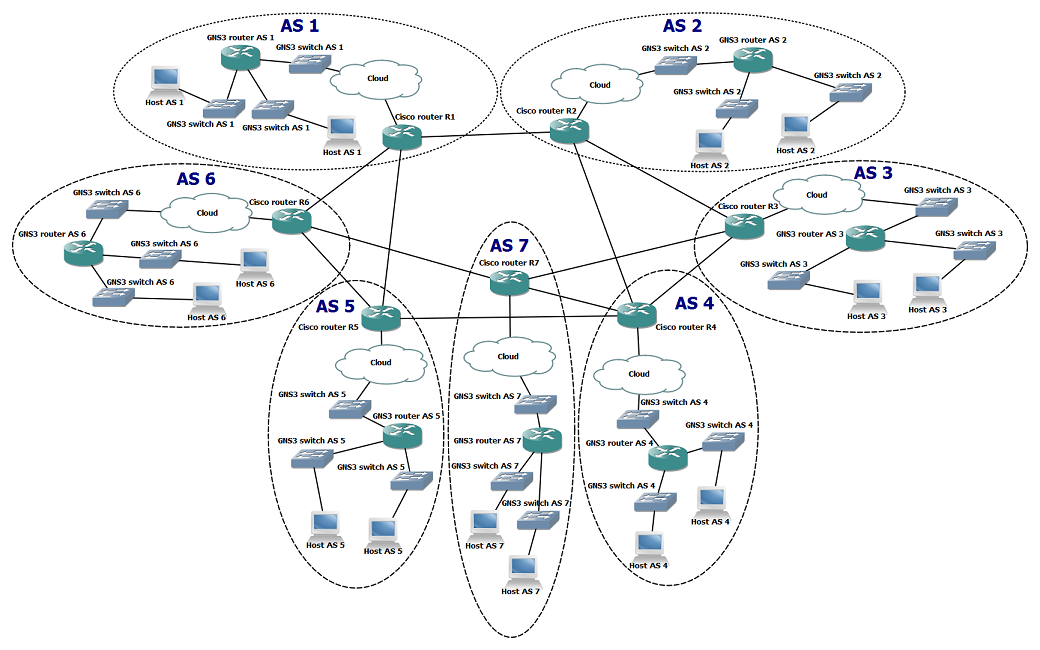
\includegraphics[width=0.9\textwidth]{figures/mini_internet.png}
    \caption{A `mini' internet topology}
    \label{fig:mini-internet}
\end{figure}

\subsection{Task}
Configure the assigned Cisco router with the IP addresses shown by Figure~\ref{fig:cisco-topo}! This exercise should
result in the desired topology.

\begin{figure}[H]
    \centering
    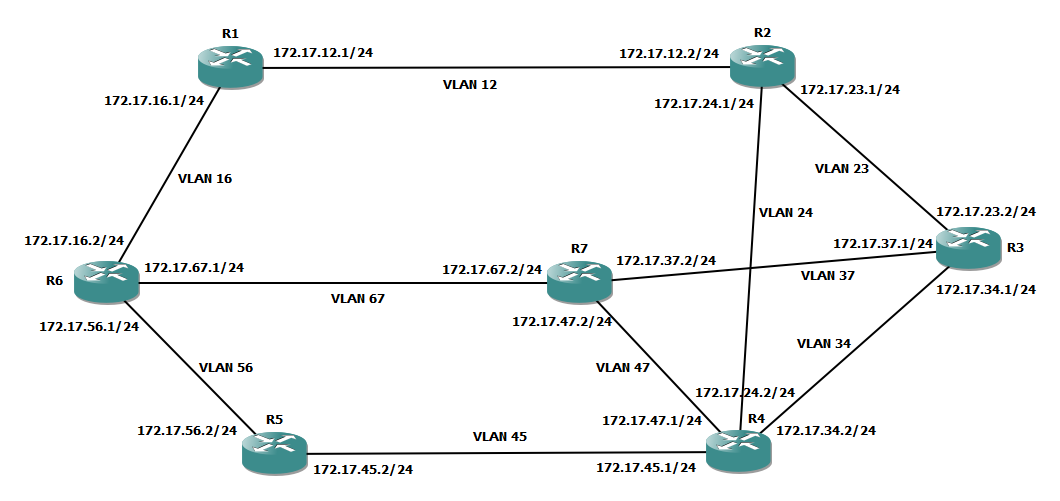
\includegraphics[width=0.9\textwidth]{figures/cisco_router_topology.png}
    \caption{Cisco routers topology}
    \label{fig:cisco-topo}
\end{figure}

\subsection{Task}

Configure the VMs in GNS3 in a way that they will have the assigned IP addresses as shown by
Figure~\ref{fig:gns3-topo}! Check the network connectivity on each link using `ping' utility. If ping is not working
somewhere explain the potential reason why it isn't working. Why does pinging Quagga router work from the host machine
but pinging the BGP (physical) router does not?

\begin{figure}[H]
    \centering
    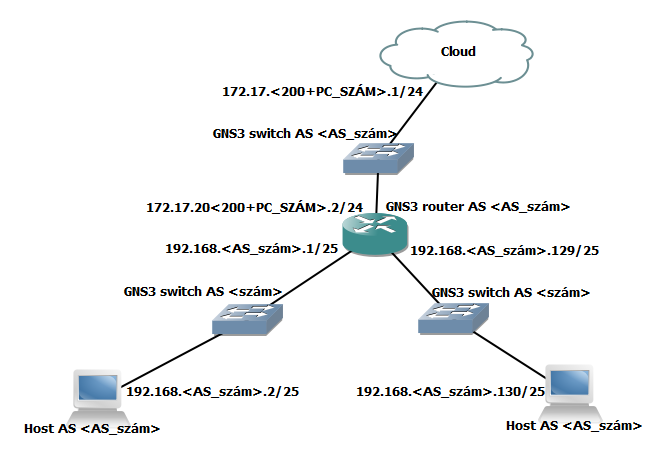
\includegraphics[width=0.9\textwidth]{figures/gns3_topology.png}
    \caption{GNS3 routers topology}
    \label{fig:gns3-topo}
\end{figure}

\subsection{Task}
Configure Quagga router so that it runs OSPF on all its internal interfaces as well as the Cisco routers. Configure the
router-id of the Quagga router.
\subsection{Task}
Configure the devices in way that the connected ASes (Autonomous Systems, marked with circle) are running eBGP protocol
between them. Form BGP neighborships between the interconnected ASBRs as shown by Figure~\ref{mini-internet} topology.
Verify and document the results!
\subsection{Task}
Configure the BGP router for automatic route redistribution from OSPF. Furthermore configure BGP for advertising 2
additional prefixes : 172.17.~\textless150+AS\_number~\textgreater.0/24 and
172.17.~\textless160+AS\_number~\textgreater.0/24. From these subnets it's advised to configure one-one on the BGP
router's loopback interface otherwise the router won't advertise the routes since it doesn't have any corresponding
routing entries. If this has been carried out by multiple groups successfully verify that their subnets are visible
from each other's AS. Verify the routes using the \emph{`traceroute'} command. Provide detailed documentation in the lab
report.
\subsection{Task}
The task is to reduce the number of entries in the routing table: Combine two arbitrarily chosen network prefix in the
routing table. Check the distribution of this route throughout the network. Document the results in the lab report.
\subsection{Task}
Configure the devices so that the connected ASBRs has to be configured to have either peer or transit connections
corresponding to the topology shown on Figure~\ref{fig:transit-connections}
\begin{figure}[H]
    \centering
    \includegraphics[width=0.9\textwidth]{figures/transit-peer-connections.png}
    \caption{Transit-peer connections}
    \label{fig:transit-connections}
\end{figure}
\subsection{Task}
Verify Valley-free routes between ASes. Chose 3 AS arbitrarily that have 2,3,4 --in order-- distance in terms of ASes.
If a valley-free route exists document it otherwise provide and document an explanation on why there isn't a
valley-free route exist towards the given AS.
\subsection{Task}
Configure the BGP import/export filters so that the neighbouring AS only receives BGP advertisements from valley-free
routes. Figure~\ref{fig:valley-free} provides help on this task. If all routes has become valley-free document that
with pictures.

\begin{figure}[H]
    \centering
    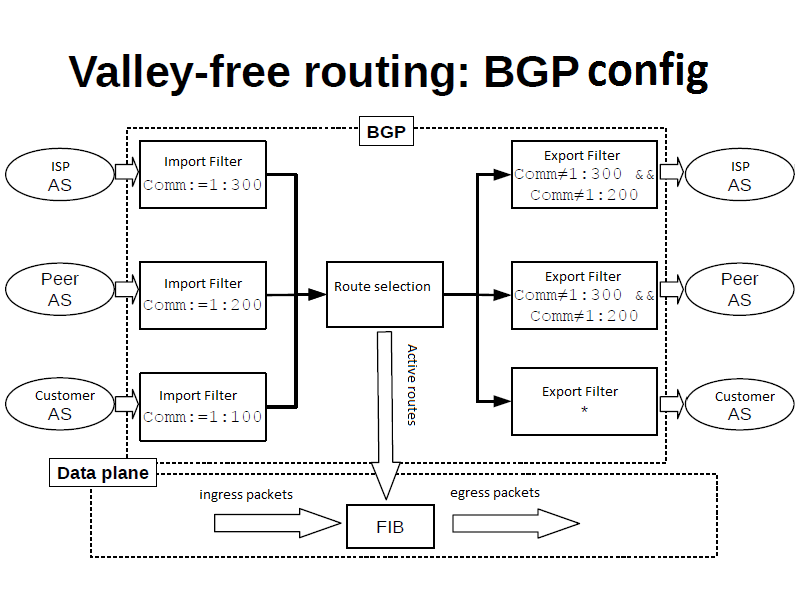
\includegraphics[width=0.9\textwidth]{figures/valley.PNG}
    \caption{Valley-free routing}
    \label{fig:valley-free}
\end{figure}

\subsection{Task}
The next task is to configure a `prefer customer' rule (hints are shown by Figure~\ref{fig:prefer-customer}).
\begin{figure}[H]
    \centering
    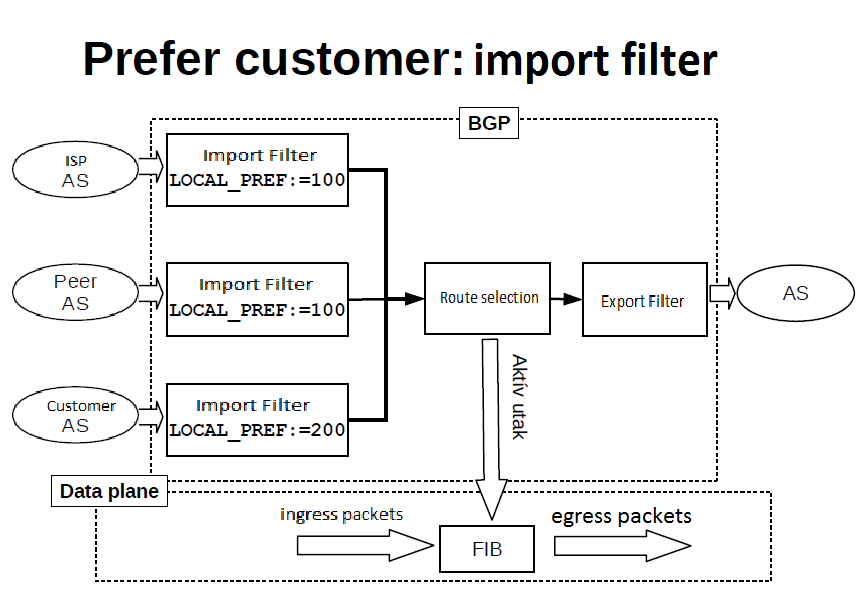
\includegraphics[width=0.9\textwidth]{figures/prefer.png}
    \caption{Prefer customer}
    \label{fig:prefer-customer}
\end{figure}

\end{document}